\documentclass[11pt,a4paper]{article}
\usepackage[margin=0.55in]{geometry}
\usepackage{amsmath,amssymb}
\usepackage{xcolor}
\usepackage{tabularx}
\usepackage{array}
\usepackage{tikz}
\usetikzlibrary{shapes.geometric,arrows.meta,positioning,calc}
\usepackage{times}

\pagestyle{empty}

\begin{document}

\begin{center}
{\LARGE \textbf{4.4\quad Overall end-to-end System flow}}\\[1.0em]
{\huge \textbf{PrismSpace Architecture}}\\[1.2em]

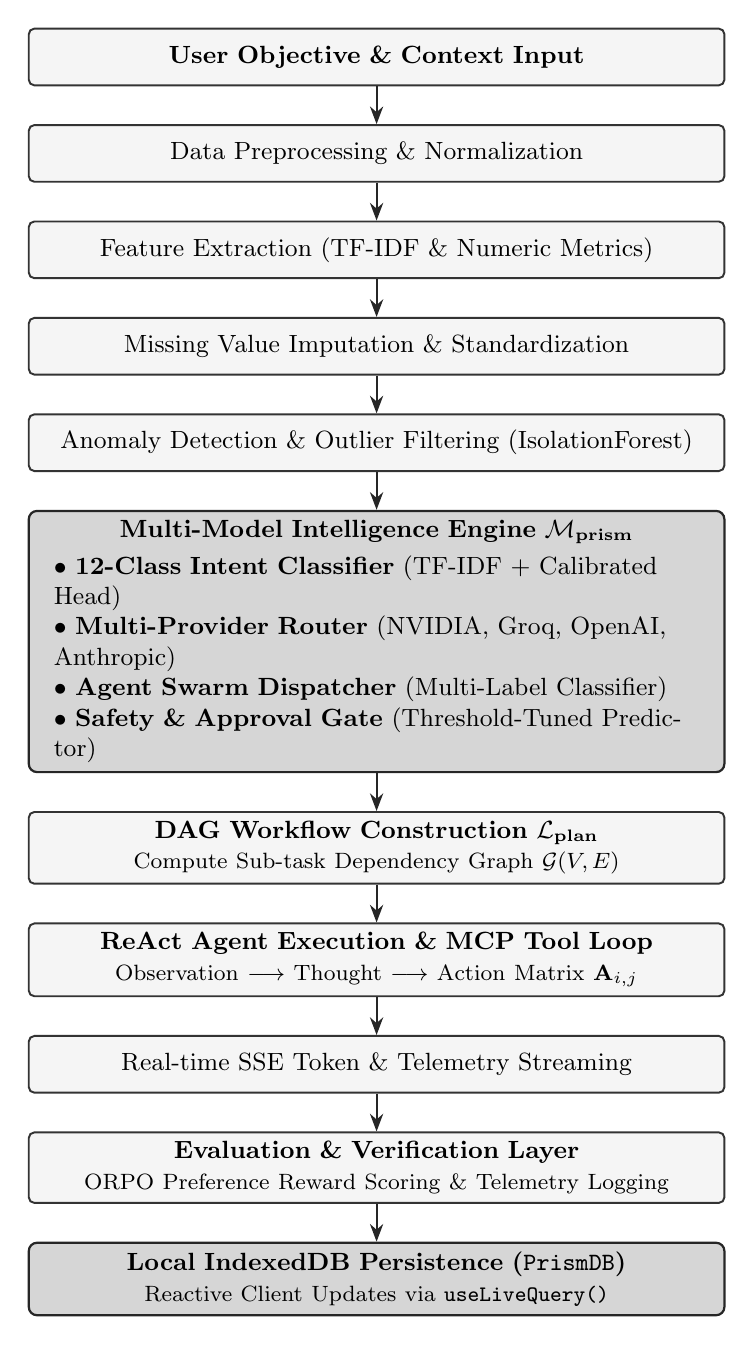
\begin{tikzpicture}[
    auto,
    node distance = 0.48cm,
    block/.style = {
        rectangle,
        draw=black!80,
        line width=0.7pt,
        fill=black!4,
        rounded corners=2pt,
        text width=8.6cm,
        minimum height=0.72cm,
        text centered,
        font=\small
    },
    shaded_block/.style = {
        rectangle,
        draw=black!85,
        line width=0.8pt,
        fill=black!16,
        rounded corners=3pt,
        text width=8.6cm,
        minimum height=1.55cm,
        align=center,
        font=\small
    },
    arrow/.style = {
        -{Stealth[scale=1.0]},
        line width=0.75pt,
        draw=black!85
    }
]

    % Node Definitions
    \node [block] (input) {\textbf{User Objective \& Context Input}};
    
    \node [block, below=of input] (prep) {Data Preprocessing \& Normalization};
    
    \node [block, below=of prep] (feat) {Feature Extraction (TF-IDF \& Numeric Metrics)};
    
    \node [block, below=of feat] (impute) {Missing Value Imputation \& Standardization};
    
    \node [block, below=of impute] (anomaly) {Anomaly Detection \& Outlier Filtering (IsolationForest)};
    
    \node [shaded_block, below=of anomaly] (ml_engine) {
        \textbf{Multi-Model Intelligence Engine $\mathcal{M}_{\text{prism}}$}\\[0.35em]
        \parbox{8.2cm}{\small
        $\bullet$ \textbf{12-Class Intent Classifier} (TF-IDF + Calibrated Head)\\
        $\bullet$ \textbf{Multi-Provider Router} (NVIDIA, Groq, OpenAI, Anthropic)\\
        $\bullet$ \textbf{Agent Swarm Dispatcher} (Multi-Label Classifier)\\
        $\bullet$ \textbf{Safety \& Approval Gate} (Threshold-Tuned Predictor)}
    };
    
    \node [block, below=of ml_engine] (graph_const) {
        \textbf{DAG Workflow Construction $\mathcal{L}_{\text{plan}}$}\\
        \footnotesize Compute Sub-task Dependency Graph $\mathcal{G}(V, E)$
    };
    
    \node [block, below=of graph_const] (react_loop) {
        \textbf{ReAct Agent Execution \& MCP Tool Loop}\\
        \footnotesize Observation $\longrightarrow$ Thought $\longrightarrow$ Action Matrix $\mathbf{A}_{i,j}$
    };
    
    \node [block, below=of react_loop] (stream) {Real-time SSE Token \& Telemetry Streaming};
    
    \node [block, below=of stream] (eval_layer) {
        \textbf{Evaluation \& Verification Layer}\\
        \footnotesize ORPO Preference Reward Scoring \& Telemetry Logging
    };
    
    \node [shaded_block, below=of eval_layer, minimum height=0.85cm] (persist) {
        \textbf{Local IndexedDB Persistence (\texttt{PrismDB})}\\
        \footnotesize Reactive Client Updates via \texttt{useLiveQuery()}
    };

    % Arrows connecting nodes
    \draw [arrow] (input) -- (prep);
    \draw [arrow] (prep) -- (feat);
    \draw [arrow] (feat) -- (impute);
    \draw [arrow] (impute) -- (anomaly);
    \draw [arrow] (anomaly) -- (ml_engine);
    \draw [arrow] (ml_engine) -- (graph_const);
    \draw [arrow] (graph_const) -- (react_loop);
    \draw [arrow] (react_loop) -- (stream);
    \draw [arrow] (stream) -- (eval_layer);
    \draw [arrow] (eval_layer) -- (persist);

\end{tikzpicture}

\vspace{1.2em}
{\Large \textbf{Figure 4.3: System flow}}
\end{center}

\vspace{0.8em}
\noindent\fcolorbox{black!50}{black!2}{%
\parbox{\dimexpr\textwidth-2\fboxsep-2\fboxrule\relax}{%
\small
\textbf{\large System Flow Glossary \& Terminology Reference}\\[0.4em]
\begin{tabular}{@{}p{0.48\linewidth}@{\hspace{0.03\linewidth}}p{0.48\linewidth}@{}}
\textbf{TF-IDF}: Term Frequency--Inverse Document Frequency; statistical metric evaluating token relevance in user queries. &
\textbf{ReAct}: Reasoning and Acting; loop alternating explicit chain-of-thought rationale with concrete tool actions.\\

\textbf{IsolationForest}: Unsupervised decision tree ensemble identifying anomalous or out-of-distribution user inputs. &
\textbf{MCP}: Model Context Protocol; open protocol enabling LLMs to safely invoke local/remote tools and data sources.\\

\textbf{$\mathcal{M}_{\text{prism}}$}: Multi-Model Intelligence Engine; dynamically routes sub-tasks across Groq, NVIDIA, OpenAI, etc. &
\textbf{SSE}: Server-Sent Events; HTTP streaming standard pushing real-time LLM token streams and execution telemetry.\\

\textbf{Safety \& Approval Gate}: Calibrated classifier halting execution for human approval on high-risk operations. &
\textbf{ORPO}: Odds Ratio Preference Optimization; reference-free preference alignment optimizing response quality.\\

\textbf{DAG $\mathcal{G}(V,E)$}: Directed Acyclic Graph; orders execution plan where vertices $V$ are tasks and edges $E$ are dependencies. &
\textbf{PrismDB / \texttt{useLiveQuery}}: Client-side IndexedDB database offering reactive, zero-latency UI re-rendering on updates.
\end{tabular}
}}

\end{document}
